\section{Техническое задание}
\subsection{Основание для разработки}

Основанием для разработки является задание по курсовой работе "<Разработка системы тестирования \textquotedbl">.

\subsection{Цель и назначение разработки}

Основной задачей курсовой работы является разработка системы тестирования для измерения качеств и свойств личности.

Задачами данной разработки являются:
\begin{itemize}
\item создание окон для редактирования вопросов;
\item создание окон для авторизации и прохождения тестов;
\item создание окон для просмотра результатов пройденных тестов;
\item реализация системы диагнозов по результатам теста;
\item реализация калькулятора расчета диагноза;
\item реализация системы хранения тестов и результатов тестов;
\end{itemize}

\subsection{Требования пользователя к интерфейсу системы тестирования}

Система должна включать в себя:
\begin{itemize}
    \item навигацию по разделам;
    \item авторизацию;
    \item возможность редактирования тестов и создания новых;
    \item возможность просмотра статистики пройденных тестов.
\end{itemize}

Композиция шаблона системы представлена на рисунке ~\ref{templ:image}.

\begin{figure}[ht]
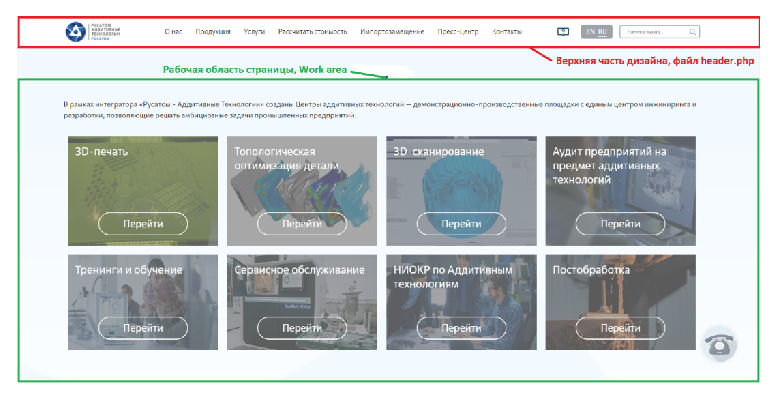
\includegraphics[width=1\linewidth]{templ}
\caption{Композиция шаблона системы}
\label{templ:image}
\end{figure}
%\vspace{-\figureaboveskip} % двойной отступ не нужен (можно использовать, если раздел заканчивается картинкой)

\subsection{Моделирование вариантов использования}

Для разрабатываемой системы тестирования была реализована модель, которая обеспечивает наглядное представление вариантов использования системы.

Она помогает в физической разработке и детальном анализе взаимосвязей объектов. При построении диаграммы вариантов использования применяется унифицированный язык визуального моделирования UML.

Диаграмма вариантов описывает функциональное назначение разрабатываемой системы. То есть это то, что система будет непосредственно делать в процессе своего функционирования. Она является исходным концептуальным представлением системы в процессе ее проектирования и разработки. Проектируемая система представляется в виде ряда прецедентов, предоставляемых системой актерам или сущностям, которые взаимодействуют с системой. Актером или действующим лицом является сущность, взаимодействующая с системой извне (например, человек, техническое устройство). Прецедент служит для описания набора действий, которые система предоставляет актеру.

На основании анализа предметной области в программе должны быть реализованы следующие прецеденты:
\begin{enumerate}
\item Просмотр информации о имеющихся тестах.
\item Просмотр информации о содержимом тесте.
\item Просмотр информации о результатах пройденных тестов.
\item Создание или редактирование тестов.
\item Прохождение тестирования.
\end{enumerate}

\subsection{Требования к оформлению документации}

Разработка программной документации и программного изделия должна производиться согласно ГОСТ 19.102-77 и ГОСТ 34.601-90. Единая система программной документации.
